\documentclass[10pt,UTF8]{ctexart}


\usepackage[margin=2cm,a4paper]{geometry}
%\usepackage[left=0.75in,top=0.6in,right=0.75in,bottom=1.0in,a4paper]{geometry}

\setmainfont{Caladea}
%% 也可以選用其它字庫:
% \setCJKmainfont[%
%   ItalicFont=AR PL KaitiM GB,
%   BoldFont=Noto Sans CJK SC,
% ]{Noto Serif CJK SC}
% \setCJKsansfont{Noto Sans CJK SC}
% \renewcommand{\kaishu}{\CJKfontspec{AR PL KaitiM GB}}

% 繁體中文
\setCJKmainfont[Path=fonts/ ]{NotoSansTC-Medium.otf}

\usepackage{minted}
\usepackage[breaklinks]{hyperref}

% Picture
% 導言區的此三行無變化
\usepackage{graphicx}
\usepackage{float} 
\usepackage{subfigure}
% 以下是新增的自定義格式更改
\usepackage[]{caption2} %新增調用的宏包
\renewcommand{\figurename}{Fig.} %重定義編號前綴詞
\renewcommand{\captionlabeldelim}{.~} %重定義分隔符
 %\roman 是羅馬數字編號,\alph是默認的字母編號,\arabic是阿拉伯數字編號,可按需替換下一行的相應位置
\renewcommand{\thesubfigure}{(\roman{subfigure})}%此外,還可設置圖編號顯示格式,加括號或者不加括號
\makeatletter \renewcommand{\@thesubfigure}{\thesubfigure \space}%子圖編號與名稱的間隔設置
\renewcommand{\p@subfigure}{} \makeatother

% Math
\usepackage {mathtools}
\usepackage{amssymb}

% Code
\usepackage{listings}
\usepackage{xcolor}
\lstset{
    % backgroundcolor=\color{red!50!green!50!blue!50},
    % 程式碼塊背景色為淺灰色
    rulesepcolor= \color{gray}, % 程式碼塊邊框顏色
    breaklines=true,  % 程式碼過長則換行
    numbers=left, % 行號在左側顯示
    numberstyle= \small,% 行號字型
    % eywordstyle= \color{red,% 關鍵字顏色
    commentstyle=\color{gray}, % 註釋顏色
    frame=shadowbox % 用方框框住程式碼塊
    }

\usepackage{hyperref}

\title{數字媒體軟件與系統開發}
\author{干皓丞,2101212850, 信息工程學院}

\begin{document}
\maketitle


\section{作業目標與章節摘要}

下載 GPAC,理解並描述 random access 過程。

\begin{figure}[H]
\centering 

\includegraphics[width=0.80\textwidth]{g2.png} 
\caption{使用安裝好的 GPAC 的 Osmo4 播放}
\label{Test}
\end{figure}


\section{文章與作業狀況}

作業可以從 GitHub 下的 kancheng/kan-cs-report-in-2022 專案找到,作業程式碼與文件目錄為 kan-cs-report-in-2022/DMSASD/gpac-random-access。實際執行的環境與實驗設備為 Google 的 Colab 、MacBook Pro (Retina, 15-inch, Mid 2014) 、 Acer Aspire R7 與 HP Victus (Nvidia GeForce RTX 3060)。


\section{作業內容概述}

此作業分二大部分,第一部分說明 GPAC 使用與理解,第二部分則描述描述 Random Access 過程。

1. GPAC 使用與理解

2. 描述 Random Access 過程

\section{GPAC 使用與理解}

GPAC 是一個 LGPL v2.1 且在大多數情況下也可以在商業許可下使用的開源多媒體框架,其專案提供了使用者在處理、檢查、打包、流式傳輸、播放和與媒體內容交互的工具。此類內容可以為音頻、影像、字幕、元數據、可縮放圖形、加密媒體、2D/3D 圖形和 ECMAScript 等任意組合。GPAC 以其廣泛的 MP4/ISOBMFF 功能而聞名,深受影像愛好者、學術研究人員、標準化機構和專業廣播公司的歡迎。

前往 GPAC (https://gpac.wp.imt.fr/) 下載,安裝後即可以使用。開啟終端機查看版本。

1. GPAC 的官方開發文件: https://doxygen.gpac.io/

2. GPAC 的 Wiki: https://github.com/gpac/gpac/wiki/Howtos

\begin{figure}[H]
\centering 
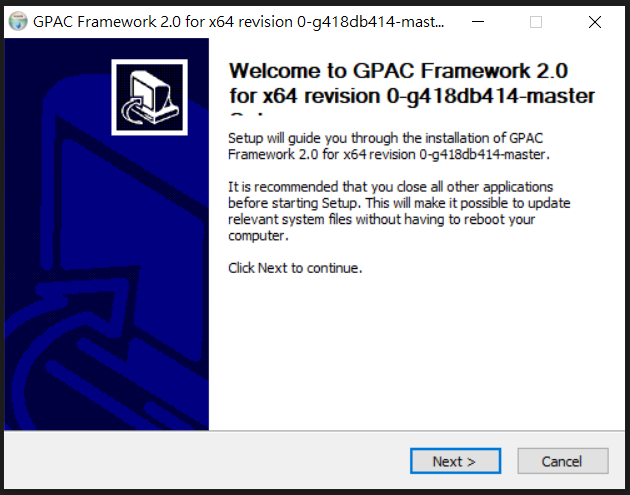
\includegraphics[width=0.80\textwidth]{g1.png} 
\caption{在此使用 GPAC 的 Windows 版本安裝}
\label{Test}
\end{figure}

\begin{figure}[H]
\centering 

\includegraphics[width=0.80\textwidth]{g2.png} 
\caption{完成}
\label{Test}
\end{figure}

1. 查看 mp4box 版本

\begin{lstlisting}[language={python}]
mp4box -version
\end{lstlisting}

\begin{figure}[H]
\centering 
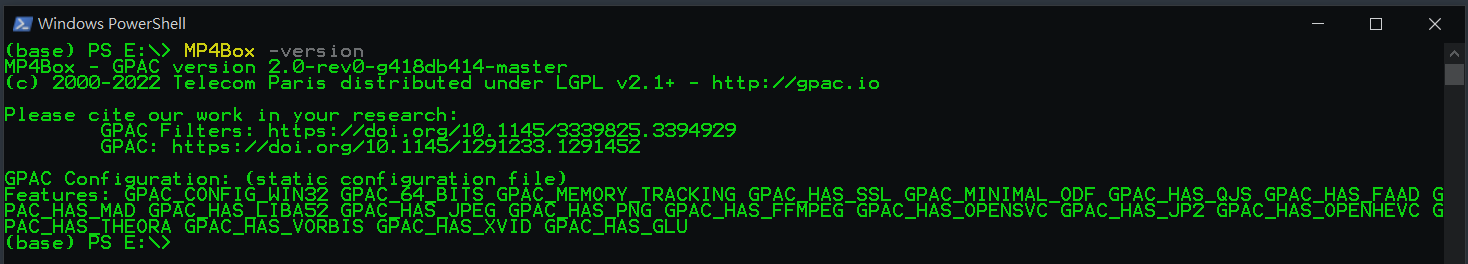
\includegraphics[width=0.80\textwidth]{g3.png} 
\caption{查看 GPAC 的  mp4box 版本}
\label{Test}
\end{figure}

2. 查看 mp4box 操作指令

\begin{lstlisting}[language={python}]
# 1
mp4box -h
# 查看 mp4box 中的所有幫助信息

# 2
mp4box -h general
# 查看 mp4box 中的通用幫助信息

# 3
mp4box -info test.mp4 
# 查看 test.mp4 文件是否有問題

# 4
mp4box -add test.mp4 test-new.mp4
# 修復 test.mp4 文件格式不標準的問題,並把新文件保存在 test-new.mp4 中

# 5
mp4box  -inter  10000 test-new.mp4 
# 解決開始播放 test-new.mp4 卡一下的問題,為 HTTP 下載快速播放有效,10000ms

# 6
mp4box -add file.avi new_file.mp4
# 把 avi 文件轉換為 mp4 文件

# 7
mp4box -hint file.mp4 
# 為 RTP 準備,此指令將為文件創建RTP提示跟踪信息。
# 這使得經典的流媒體服務器像 darwinstreamingserver 或 QuickTime 的流媒體服務器通過 RTSP/RTP 傳輸文件

# 8
mp4box -cat test1.mp4 -cat test2.mp4 -new test.mp4 
# 把 test1.mp4 和 test2.mp4 合併到一個新的文件 test.mp4 中,要求編碼參數一致

# 9
mp4box -force-cat test1.mp4 -force-cat test2.mp4 -new test.mp4 
# 把 test1.mp4 和 test2.mp4 強制合併到一個新的文件 test.mp4 中,有可能不能播放

# 10
mp4box -add video1.264 -cat video2.264 -cat video3.264 -add audio1.aac -cat audio2.aac -cat audio3.aac -new muxed.mp4 -fps 24 
# 合併多段音視頻並保持同步 

# 11
mp4box -split *time_sec* test.mp4
# 切取 test.mp4 中的前面 time_sec 秒的視頻文件

# 12
mp4box -split-size *size *test.mp4 
# 切取前面大小為 size KB的視頻文件

# 13
mp4box -split-chunk *S:E* test.mp4 
# 切取起始為 S 少,結束為 E 秒的視頻文件

# 14
mp4box -add 1.mp4#video -add 2.mp4#audio -new test.mp4
# test.mp4 由 1.mp4 中的視頻與 2.mp4 中的音頻合併生成
\end{lstlisting}

\section{描述 Random Access 過程}


\begin{figure}[H]
\centering 
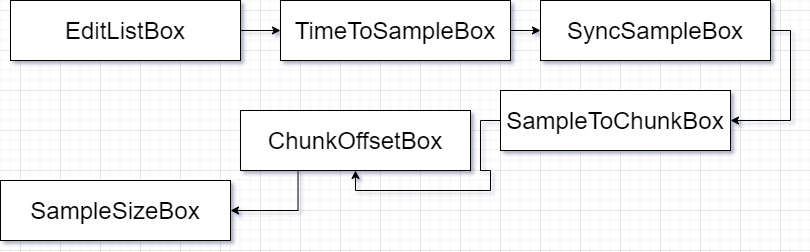
\includegraphics[width=0.80\textwidth]{g8.png} 
\caption{描述 Random Access 過程圖}
\label{Test}
\end{figure}

If you want to seek a given track to a time T,

假如想要最一個文件進行隨機訪問,而該訪問進行為 T 時刻 EX : 第三分五十秒。

1. If the track contains an edit list, determine which edit contains the time T by iterating over the edits. T\_movie = T\_start + T’

如果軌道包含編輯列表,則通過迭代編輯確定哪個編輯包含時間 T。 T\_movie = T\_start + T'

先找當中有沒有 edit list,當中 edit list 實際上存著一段段的樣本信息,這裡面會有一個關鍵字段的有開始時刻(T\_start)的連續樣本。這個過程就是將 T 換算成 T\_start + T',而這個 T' 就是換算出來的新的時間。

2. Convert to media time scale T\_media = T\_start’ + T’’

然後再將原先的過程轉換為媒體時間尺度 T\_media = T\_start' + T''


3. Use time-to-sample box to find the first sample prior to the given time

使用 time-to-sample box 找到給定時間之前的第一個樣本,也就是對應的樣本編號。

4. Consult the sync sample table to seek to which sample is closest to, but prior to, the sample found above

因為找到的樣本不一定是可以解的,為了保險會先查閱同步樣本表以尋找最接近但先於上面所找到的樣本的樣本編號。

5. Use the sample-to-chunk table to determine in which chunk this sample is located.

使用 sample-to-chunk 來確定該樣本位於哪個 chunk 中。

6. use the chunk offset box to figure out where that chunk begins

找到後根據使用 the chunk offset box 來確定該 chunk 開始的物理存儲位置。

7. Starting from this offset, you can use the information contained in the sample-to-chunk box and the sample size box to figure out where within this chunk the sample in question is located.

從這個偏移量開始,您可以使用包含在 sample-to-chunk box 和 the sample size box 中的信息來確定有問題的樣本在這個 chunk 中的位置。

尋找專案中有關 Random Access 的部分,利用 find 和 grep 指令,尋找 GPAC 與 Random Access 過程有關的檔案。


\begin{lstlisting}[language={python}]
find . -name "*.*" |xargs grep "random access" *.*
\end{lstlisting}

\begin{figure}[H]
\centering 
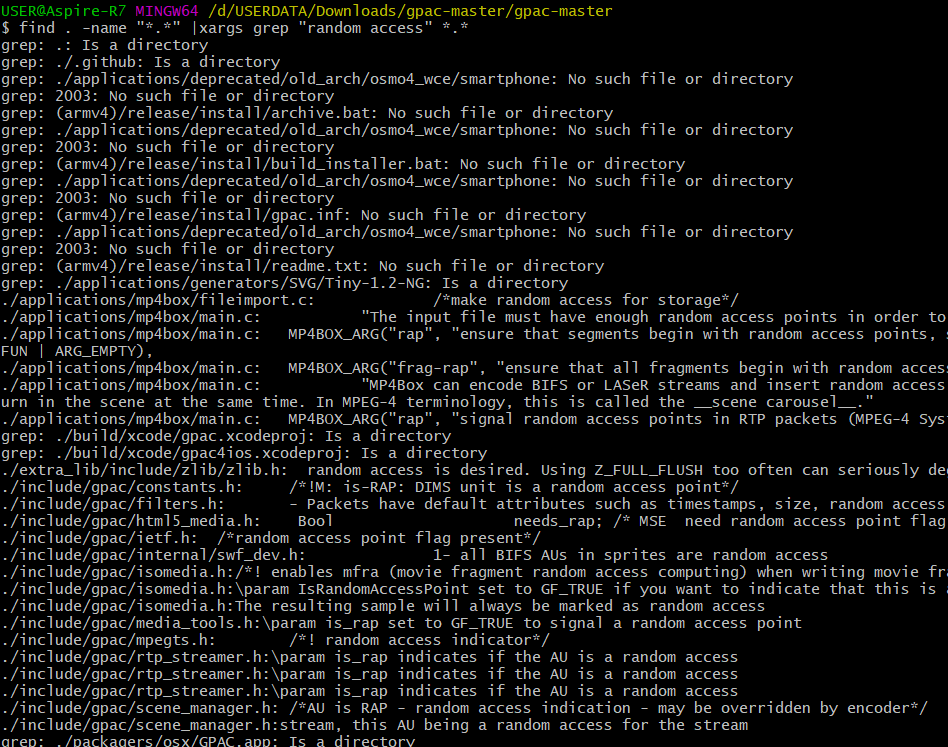
\includegraphics[width=0.80\textwidth]{g6.png} 
\caption{尋找 GPAC 與 Random Access 過程有關的檔案}
\label{Test}
\end{figure}

\begin{lstlisting}[language={python}]
./applications/mp4box/fileimport.c
./applications/mp4box/main.c
./extra_lib/include/zlib/zlib.h
./include/gpac/constants.h
./include/gpac/filters.h:
./include/gpac/html5_media.h:
./include/gpac/ietf.h:
./include/gpac/internal/swf_dev.h:
./include/gpac/isomedia.h:
./include/gpac/isomedia.h:
./include/gpac/media_tools.h:
./include/gpac/mpegts.h:
./include/gpac/rtp_streamer.h:
./include/gpac/scene_manager.h: 
./share/doc/man/gpac-filters.1:mfra (bool, default: false):
./share/doc/man/mp4box.1:
./src/filters/mux_isom.c:
./src/media_tools/html5_mse.c: 
./src/media_tools/m2ts_mux.c:
./src/scene_manager/text_to_bifs.c:
\end{lstlisting}

同時可以從 GPAC 的官方文件看到 Random Access 的部分。

\begin{figure}[H]
\centering 
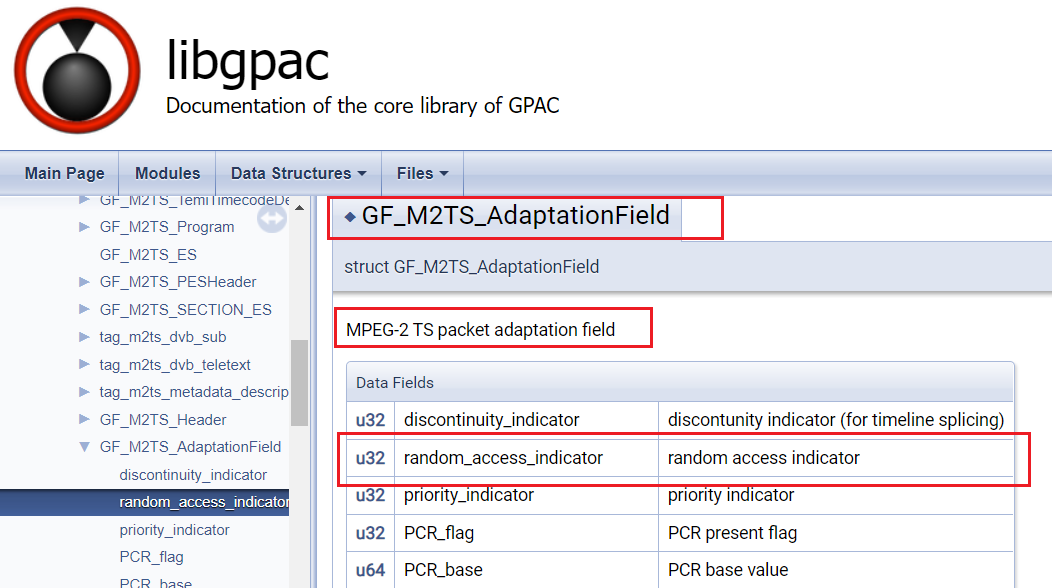
\includegraphics[width=0.80\textwidth]{g7.png} 
\caption{文件 GPAC 與 Random Access }
\label{Test}
\end{figure}

0. MP4 架構分析 - MP4Box.js

https://github.com/gpac/mp4box.js

這個JavaScript 庫可以在瀏覽器(和 node.js 中)處理 mp4 ⽂件,並⽀持解析。靈感來⾃ GPAC 項⽬中的 MP4Box⼯具。它可以⽤來:
獲取有關 mp4⽂件的信息,將 mp4⽂件分段,以便與媒體源擴展 API ⼀起使⽤,從 mp4 中提取樣本來創建 TextTracks。其提供了⼀個線上分析MP4的⽹站,可以對 MP4 進⼀步的解析,並且更直觀的幫助我們了解此次的作業內容。 ⾸先可以看⻅對這個檔案的 overview,也是兩個 Track。

https://gpac.github.io/mp4box.js/test/filereader.html

\begin{figure}[H]
\centering 
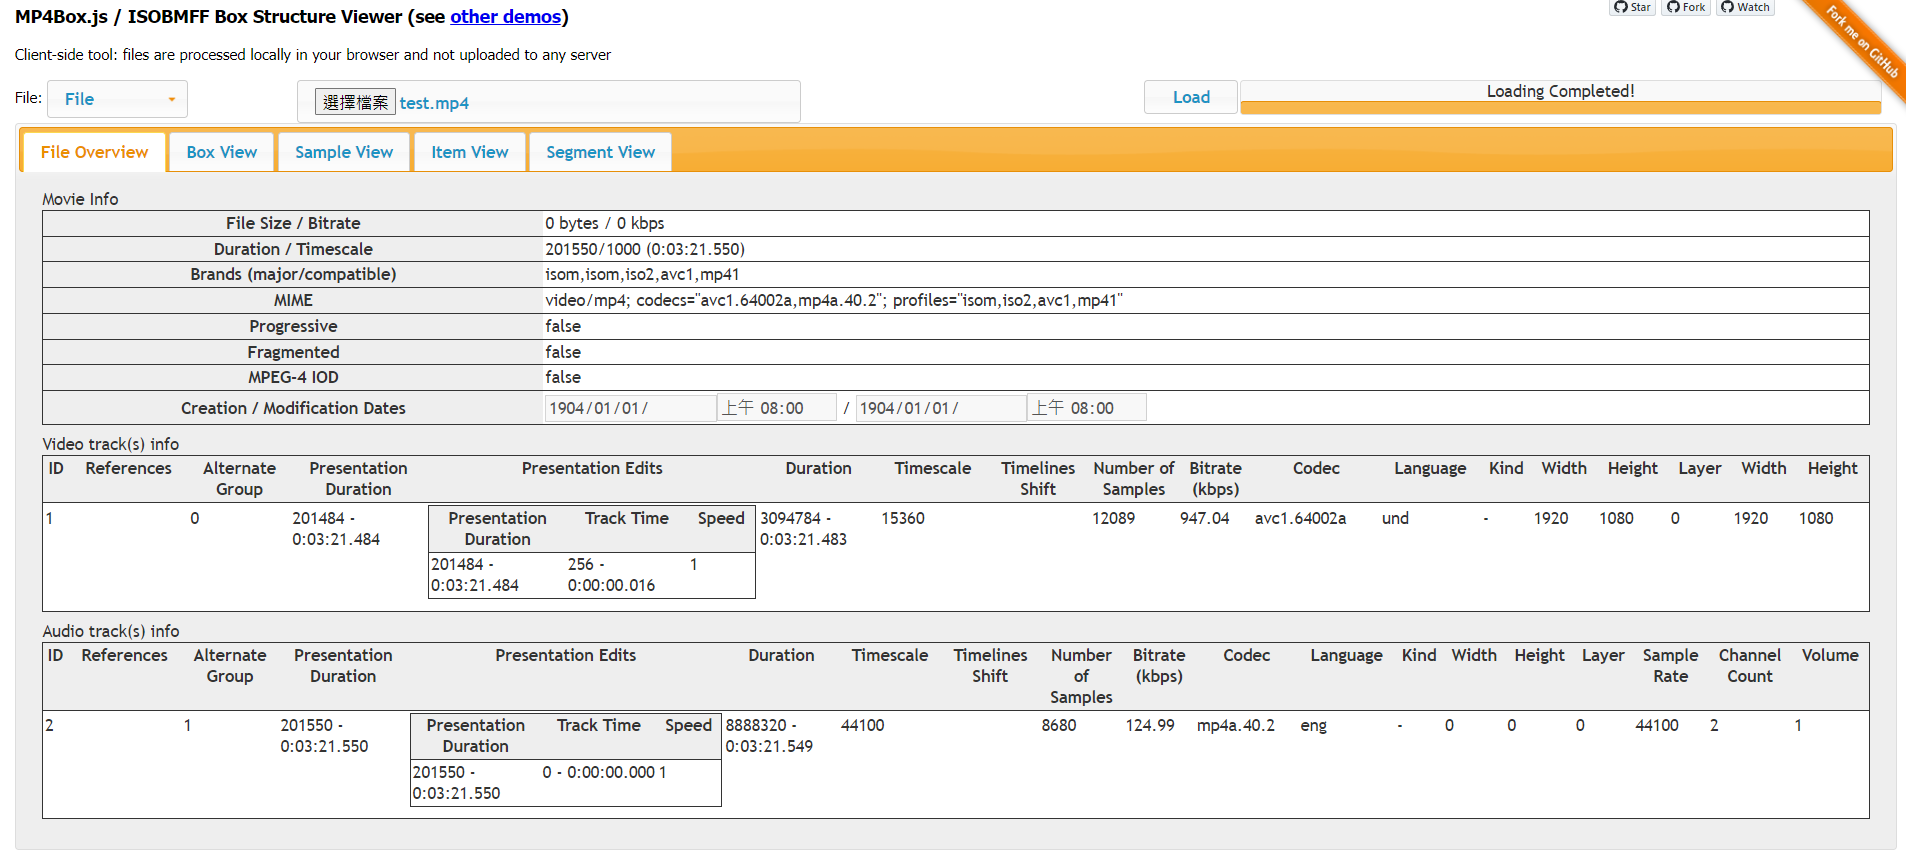
\includegraphics[width=0.80\textwidth]{m1.png} 
\caption{MP4 架構分析 }
\label{Test}
\end{figure}

\begin{figure}[H]
\centering 
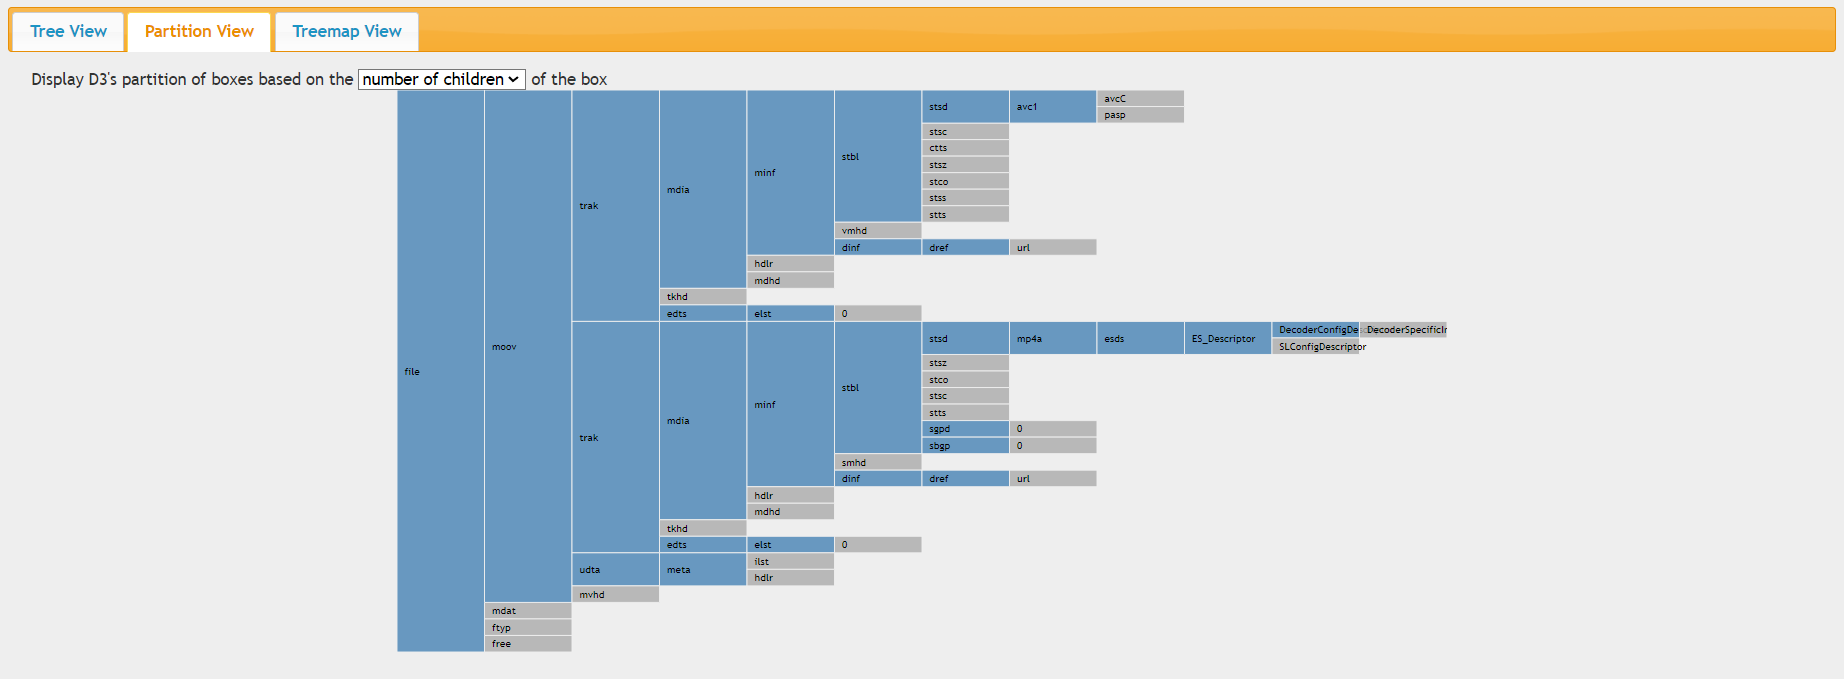
\includegraphics[width=0.80\textwidth]{m2.png} 
\caption{MP4 架構分析 }
\label{Test}
\end{figure}


\begin{figure}[H]
\centering 
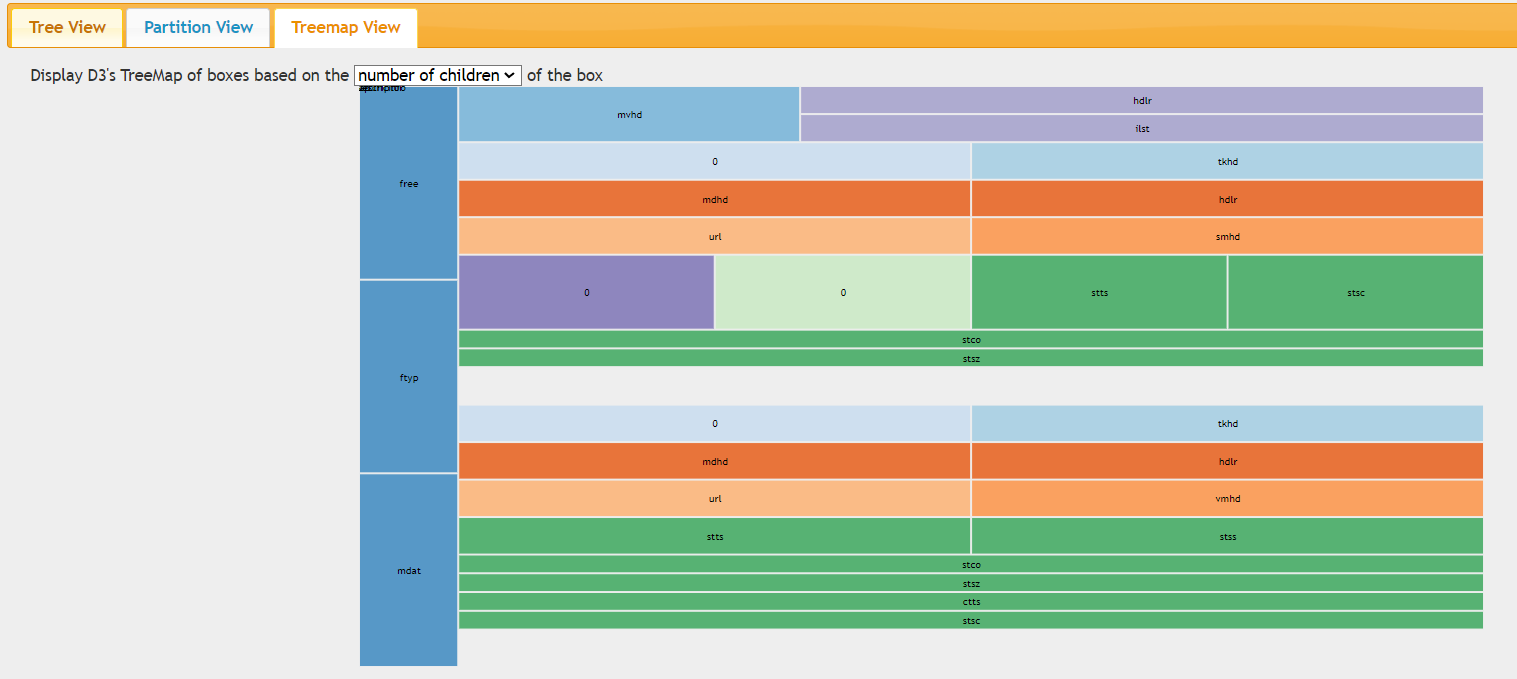
\includegraphics[width=0.80\textwidth]{m3.png} 
\caption{MP4 架構分析 }
\label{Test}
\end{figure}


1. 技術文件

本節描述如何尋找。查找主要通過使⽤ sample table box 中的⼦ box 來完成。如果 edit list 存在,也必須查閱它。 如果你想尋找⼀個給定的軌道到⼀個時間 T,其中 T 是movie header box的time scale,執⾏以下操作:

\begin{lstlisting}[language={python}]
1. If the track contains an edit list, determine which edit contains the time T by iterating over the edits. The start time of the edit in the movie time scale must then be subtracted from the time T to generate T', the duration into the edit in the movie time scale. T' is next converted to the time scale of the track's media to generate T''. Finally, the time in the media scale to use is calculated by adding the media start time of the edit to T''.

(如果track有edit list,遍歷所有edit,找到T在哪⼀個track⾥。將edit的開始時間轉換為 movie 的 time scale為單位得到edit_T,T減去edit_T,得到T',也就是在edit ⾥⾯的持續時間。將T'轉換成 track媒體 的time scale,得到T''。最後將T''加上edit_T,可以得到以 track 媒體 的time scale為單位的T''',⽽這個T'''就是後續⽤來求sample的時間)
2. The time-to-sample box for a track indicates what times are associated with which sample for that track. Use this box to find the first sample prior to the given time. EditListBox TimeToSampleBox SyncSampleBox SampleToChunkBox ChunkOffsetBox SampleSizeBox
3. The sample that was located in step 1 may not be a random access point. Locating the nearest random access point requires consulting two boxes. The sync sample table indicates which samples are in fact random access points. Using this table, you can locate which is the first sync sample prior to the specified time. The absence of the sync sample table indicates that all samples are synchronization points, and makes this problem easy. The shadow sync box gives the opportunity for a content author to provide samples that are not delivered in the normal course of delivery, but which can be inserted to provide additional random access points. This improves random access without impacting bitrate during normal delivery. This box maps samples that are not random access points to alternate samples
that are. You should also consult this table if present to find the first shadow sync sample prior to the sample in question. Having consulted the sync sample table and the shadow sync table, you probably wish to seek to whichever resultant sample is closest to, but prior to, the sample found in step 1.
4. At this point you know the sample that will be used for random access. Use the sample-to-chunk table to determine in which chunk this sample is located.
5. Knowing which chunk contained the sample in question, use the chunk offset box to figure out where that chunk begins.
6. Starting from this offset, you can use the information contained in the sample-to-chunk box and the sample size box to figure out where within this chunk the sample in question is located. This is the desired information.
\end{lstlisting}

2. 程式碼分析 MP4Box

Random Access主要看以下兩個檔案 isom\_read.c 、 stbl\_read.c

\begin{lstlisting}[language={python}]
/……/gpac-master/src/isomedia/isom\_read.c

/……/gpac-master/src/isomedia/stbl\_read.c
\end{lstlisting}

其中,對於時間T的轉換,並且獲得相應的time scale位於第⼀個 isom\_read.c ⾥⾯。⽽在各個box中尋找sample、chunk、offset……等,位於第⼆個 stbl\_read.c 中。Step1、 將時間已經轉化為 media time scale 單位,且獲得sample。

isom\_read.c 具體如下:

\begin{lstlisting}[language={python}]
//return the timescale of the movie, 0 if error
GF_EXPORT
u32 gf_isom_get_timescale(GF_ISOFile *movie)
{
	if (!movie || !movie->moov || !movie->moov->mvhd) return 0;
	return movie->moov->mvhd->timeScale;
}


//return the duration of the movie, 0 if error
GF_EXPORT
u64 gf_isom_get_duration(GF_ISOFile *movie)
{
	if (!movie || !movie->moov || !movie->moov->mvhd) return 0;

	//if file was open in Write or Edit mode, recompute the duration
	//the duration of a movie is the MaxDuration of all the tracks...

#ifndef GPAC_DISABLE_ISOM_WRITE
	gf_isom_update_duration(movie);
#endif /*GPAC_DISABLE_ISOM_WRITE*/

	return movie->moov->mvhd->duration;
}
//return the duration of the movie, 0 if error
GF_EXPORT
u64 gf_isom_get_original_duration(GF_ISOFile *movie)
{
	if (!movie || !movie->moov|| !movie->moov->mvhd) return 0;
	return movie->moov->mvhd->original_duration;
}
\end{lstlisting}


\begin{lstlisting}[language={python}]
//Return the media time given the absolute time in the Movie
GF_EXPORT
GF_Err gf_isom_get_media_time(GF_ISOFile *the_file, u32 trackNumber, u32 movieTime, u64 *MediaTime)
{
	GF_TrackBox *trak;
	u8 useEdit;
	s64 SegmentStartTime, mediaOffset;
	trak = gf_isom_get_track_from_file(the_file, trackNumber);
	if (!trak || !MediaTime) return GF_BAD_PARAM;

	SegmentStartTime = 0;
	return GetMediaTime(trak, GF_FALSE, movieTime, MediaTime, &SegmentStartTime, &mediaOffset, &useEdit, NULL);
}


//Get the stream description index (eg, the ESD) for a given time IN MEDIA TIMESCALE
//return 0 if error or if empty
GF_EXPORT
u32 gf_isom_get_sample_description_index(GF_ISOFile *movie, u32 trackNumber, u64 for_time)
{
	u32 streamDescIndex;
	GF_TrackBox *trak;
	trak = gf_isom_get_track_from_file(movie, trackNumber);
	if (!trak) return 0;

	if ( (movie->LastError = Media_GetSampleDescIndex(trak->Media, for_time, &streamDescIndex)) ) {
		return 0;
	}
	return streamDescIndex;
}

\end{lstlisting}

\begin{lstlisting}[language={python}]
//return a sample given a desired display time IN MEDIA TIME SCALE
//and set the StreamDescIndex of this sample
//this index allows to retrieve the stream description if needed (2 media in 1 track)
//return NULL if error
//WARNING: the sample may not be sync even though the sync was requested (depends on the media)
GF_EXPORT
GF_Err gf_isom_get_sample_for_media_time(GF_ISOFile *the_file, u32 trackNumber, u64 desiredTime, u32 *StreamDescriptionIndex, GF_ISOSearchMode SearchMode, GF_ISOSample **sample, u32 *SampleNum, u64 *data_offset)
{
	GF_Err e;
	u32 sampleNumber, prevSampleNumber, syncNum, shadowSync;
	GF_TrackBox *trak;
	GF_ISOSample *shadow;
	GF_SampleTableBox *stbl;
	Bool static_sample = GF_FALSE;
	u8 useShadow, IsSync;

	if (SampleNum) *SampleNum = 0;
	trak = gf_isom_get_track_from_file(the_file, trackNumber);
	if (!trak) return GF_BAD_PARAM;

	stbl = trak->Media->information->sampleTable;

#ifndef	GPAC_DISABLE_ISOM_FRAGMENTS
	if (desiredTime < trak->dts_at_seg_start) {
		desiredTime = 0;
	} else {
		desiredTime -= trak->dts_at_seg_start;
	}
#endif

	e = stbl_findEntryForTime(stbl, desiredTime, 0, &sampleNumber, &prevSampleNumber);
	if (e) return e;
\end{lstlisting}

Step2、 接著在 stbl\_read.c 中調⽤ stbl\_findEntryForTime 函數,得到 sample 編號

\begin{lstlisting}[language={python}]
//Get the sample number
GF_Err stbl_findEntryForTime(GF_SampleTableBox *stbl, u64 DTS, u8 useCTS, u32 *sampleNumber, u32 *prevSampleNumber)
{
	u32 i, j, curSampNum, count;
	s32 CTSOffset;
	u64 curDTS;
	GF_SttsEntry *ent;
	(*sampleNumber) = 0;
	(*prevSampleNumber) = 0;

	if (!stbl->TimeToSample) return GF_ISOM_INVALID_FILE;

	/*CTS is ALWAYS disabled for now to make sure samples are fetched in decoding order. useCTS is therefore disabled*/
#if 0
	if (!stbl->CompositionOffset) useCTS = 0;
#endif

	//our cache
	if (stbl->TimeToSample->r_FirstSampleInEntry &&
	        (DTS >= stbl->TimeToSample->r_CurrentDTS) ) {
		//if we're using CTS, we don't really know whether we're in the good entry or not
		//(eg, the real DTS of the sample could be in a previous entry
		i = stbl->TimeToSample->r_currentEntryIndex;
		curDTS = stbl->TimeToSample->r_CurrentDTS;
		curSampNum = stbl->TimeToSample->r_FirstSampleInEntry;
	} else {
		i = 0;
		curDTS = stbl->TimeToSample->r_CurrentDTS = 0;
		curSampNum = stbl->TimeToSample->r_FirstSampleInEntry = 1;
		stbl->TimeToSample->r_currentEntryIndex = 0;
	}

\end{lstlisting}

Step3、在 step1 中的可能不是 random access point.,所以要找到最近的random access point

\begin{lstlisting}[language={python}]
	//if no syncTable, disable syncSearching, as all samples ARE sync
	if (! trak->Media->information->sampleTable->SyncSample) {
		if (SearchMode == GF_ISOM_SEARCH_SYNC_FORWARD) SearchMode = GF_ISOM_SEARCH_FORWARD;
		if (SearchMode == GF_ISOM_SEARCH_SYNC_BACKWARD) SearchMode = GF_ISOM_SEARCH_BACKWARD;
	}
\end{lstlisting}

\begin{lstlisting}[language={python}]
	//get the sync sample num
	if (IsSync) {
		//get the SyncNumber
		e = Media_FindSyncSample(trak->Media->information->sampleTable,
		                         sampleNumber, &syncNum, SearchMode);
		if (e) return e;
		if (syncNum) sampleNumber = syncNum;
		syncNum = 0;
	}
	//if we are in shadow mode, get the previous sync sample
	//in case we can't find a good SyncShadow
	else if (SearchMode == GF_ISOM_SEARCH_SYNC_SHADOW) {
		//get the SyncNumber
		e = Media_FindSyncSample(trak->Media->information->sampleTable,
		                         sampleNumber, &syncNum, GF_ISOM_SEARCH_SYNC_BACKWARD);
		if (e) return e;
	}
\end{lstlisting}

調⽤ stbl\_GetSampleRap 函數,找到與給定的 sample 編號最近的 RAP( random access point),如果當前 sample 就是 RAP ,則設置 RAP 這個 flag

\begin{lstlisting}[language={python}]
//Retrieve closes RAP for a given sample - if sample is RAP, sets the RAP flag
GF_Err stbl_GetSampleRAP(GF_SyncSampleBox *stss, u32 SampleNumber, GF_ISOSAPType *IsRAP, u32 *prevRAP, u32 *nextRAP)
{
	u32 i;
	if (prevRAP) *prevRAP = 0;
	if (nextRAP) *nextRAP = 0;

	(*IsRAP) = RAP_NO;
	if (!stss || !SampleNumber) return GF_BAD_PARAM;

	if (stss->r_LastSyncSample && (stss->r_LastSyncSample < SampleNumber) ) {
		i = stss->r_LastSampleIndex;
	} else {
		i = 0;
	}
	for (; i < stss->nb_entries; i++) {
		//get the entry
		if (stss->sampleNumbers[i] == SampleNumber) {
			//update the cache
			stss->r_LastSyncSample = SampleNumber;
			stss->r_LastSampleIndex = i;
			(*IsRAP) = RAP;
		}
		else if (stss->sampleNumbers[i] > SampleNumber) {
			if (nextRAP) *nextRAP = stss->sampleNumbers[i];
			return GF_OK;
		}
		if (prevRAP) *prevRAP = stss->sampleNumbers[i];
	}
	return GF_OK;
}
\end{lstlisting}

Step4、使⽤sample\_to\_chunk box找到 sample 对应的 chunk

\begin{lstlisting}[language={python}]
//get the number of "ghost chunk" (implicit chunks described by an entry)
void GetGhostNum(GF_StscEntry *ent, u32 EntryIndex, u32 count, GF_SampleTableBox *stbl)
{
	GF_StscEntry *nextEnt;
	u32 ghostNum = 1;

	if (!ent) {
		stbl->SampleToChunk->ghostNumber = 0;
		return;
	}

	if (!ent->nextChunk) {
		if (EntryIndex+1 == count) {
			//not specified in the spec, what if the last sample to chunk is no written?
			if (stbl->ChunkOffset->type == GF_ISOM_BOX_TYPE_STCO) {
				GF_ChunkOffsetBox *stco = (GF_ChunkOffsetBox *)stbl->ChunkOffset;
				ghostNum = (stco->nb_entries > ent->firstChunk) ? (1 + stco->nb_entries - ent->firstChunk) : 1;
			} else {
				GF_ChunkLargeOffsetBox *co64 = (GF_ChunkLargeOffsetBox *)stbl->ChunkOffset;
				ghostNum = (co64->nb_entries > ent->firstChunk) ? (1 + co64->nb_entries - ent->firstChunk) : 1;
			}
		} else {
			//this is an unknown case due to edit mode...
			nextEnt = &stbl->SampleToChunk->entries[EntryIndex+1];
			ghostNum = nextEnt->firstChunk - ent->firstChunk;
		}
	} else {
		ghostNum = (ent->nextChunk > ent->firstChunk) ? (ent->nextChunk - ent->firstChunk) : 1;
	}
	stbl->SampleToChunk->ghostNumber = ghostNum;
}
\end{lstlisting}

Step5、 根據 stco (ChunkOffsetBox)獲取對應 Chunk 在⽂件中的偏移位置。

\begin{lstlisting}[language={python}]
//Get the offset, descIndex and chunkNumber of a sample...
GF_Err stbl_GetSampleInfos(GF_SampleTableBox *stbl, u32 sampleNumber, u64 *offset, u32 *chunkNumber, u32 *descIndex, GF_StscEntry **out_ent)
{
	GF_Err e;
	u32 i, k, offsetInChunk, size, chunk_num;
	GF_ChunkOffsetBox *stco;
	GF_ChunkLargeOffsetBox *co64;
	GF_StscEntry *ent;

	(*offset) = 0;
	(*chunkNumber) = (*descIndex) = 0;
	if (out_ent) (*out_ent) = NULL;
	if (!stbl || !sampleNumber) return GF_BAD_PARAM;
	if (!stbl->ChunkOffset || !stbl->SampleToChunk || !stbl->SampleSize) return GF_ISOM_INVALID_FILE;

	if (stbl->SampleSize && stbl->SampleToChunk->nb_entries == stbl->SampleSize->sampleCount) {
		ent = &stbl->SampleToChunk->entries[sampleNumber-1];
		if (!ent) return GF_BAD_PARAM;
		(*descIndex) = ent->sampleDescriptionIndex;
		(*chunkNumber) = sampleNumber;
		if (out_ent) *out_ent = ent;
		if ( stbl->ChunkOffset->type == GF_ISOM_BOX_TYPE_STCO) {
			stco = (GF_ChunkOffsetBox *)stbl->ChunkOffset;
			if (!stco->offsets) return GF_ISOM_INVALID_FILE;
			if (stco->nb_entries < sampleNumber) return GF_ISOM_INVALID_FILE;

			(*offset) = (u64) stco->offsets[sampleNumber - 1];
		} else {
			co64 = (GF_ChunkLargeOffsetBox *)stbl->ChunkOffset;
			if (!co64->offsets) return GF_ISOM_INVALID_FILE;
			if (co64->nb_entries < sampleNumber) return GF_ISOM_INVALID_FILE;

			(*offset) = co64->offsets[sampleNumber - 1];
		}
		return GF_OK;
	}
\end{lstlisting}


\begin{lstlisting}[language={python}]
	//ok, get the size of all the previous samples in the chunk
	offsetInChunk = 0;
	//constant size
	if (stbl->SampleSize && stbl->SampleSize->sampleSize) {
		u32 diff = sampleNumber - stbl->SampleToChunk->firstSampleInCurrentChunk;
		offsetInChunk += diff * stbl->SampleSize->sampleSize;
	} else if ((stbl->r_last_chunk_num == chunk_num) && (stbl->r_last_sample_num == sampleNumber)) {
		offsetInChunk = stbl->r_last_offset_in_chunk;
	} else if ((stbl->r_last_chunk_num == chunk_num) && (stbl->r_last_sample_num + 1 == sampleNumber)) {
		e = stbl_GetSampleSize(stbl->SampleSize, stbl->r_last_sample_num, &size);
		if (e) return e;
		stbl->r_last_offset_in_chunk += size;
		stbl->r_last_sample_num = sampleNumber;
		offsetInChunk = stbl->r_last_offset_in_chunk;
	} else {
		//warning, firstSampleInChunk is at least 1 - not 0
		for (i = stbl->SampleToChunk->firstSampleInCurrentChunk; i < sampleNumber; i++) {
			e = stbl_GetSampleSize(stbl->SampleSize, i, &size);
			if (e) return e;
			offsetInChunk += size;
		}
		stbl->r_last_chunk_num = chunk_num;
		stbl->r_last_sample_num = sampleNumber;
		stbl->r_last_offset_in_chunk = offsetInChunk;
	}
	//OK, that's the size of our offset in the chunk
	//now get the chunk
	if ( stbl->ChunkOffset->type == GF_ISOM_BOX_TYPE_STCO) {
		stco = (GF_ChunkOffsetBox *)stbl->ChunkOffset;
		if (stco->nb_entries < (*chunkNumber) ) return GF_ISOM_INVALID_FILE;
		(*offset) = (u64) stco->offsets[(*chunkNumber) - 1] + (u64) offsetInChunk;
	} else {
		co64 = (GF_ChunkLargeOffsetBox *)stbl->ChunkOffset;
		if (co64->nb_entries < (*chunkNumber) ) return GF_ISOM_INVALID_FILE;
		(*offset) = co64->offsets[(*chunkNumber) - 1] + (u64) offsetInChunk;
	}
	return GF_OK;
}
\end{lstlisting}

Step6、根據 stsz (SampleSizeBox)獲取 Sample 在 Chunk 內的偏移位置並加上第 4 步獲取的偏移,計算出 Sample 在⽂件中的偏移。


\begin{lstlisting}[language={python}]
GF_Err stbl_SearchSAPs(GF_SampleTableBox *stbl, u32 SampleNumber, GF_ISOSAPType *IsRAP, u32 *prevRAP, u32 *nextRAP)
{
	u32 i, j, count, count2;
	assert(prevRAP);
	assert(nextRAP);
	(*prevRAP) = 0;
	(*nextRAP) = 0;
	(*IsRAP) = RAP_NO;

	if (!stbl->sampleGroups || !stbl->sampleGroupsDescription) return GF_OK;

	count = gf_list_count(stbl->sampleGroups);
	count2 = gf_list_count(stbl->sampleGroupsDescription);
	for (i=0; i<count; i++) {
		GF_SampleGroupDescriptionBox *sgdp = NULL;
		Bool is_rap_group = 0;
		s32 roll_distance = 0;
		u32 first_sample_in_entry, last_sample_in_entry;
		GF_SampleGroupBox *sg = gf_list_get(stbl->sampleGroups, i);
		switch (sg->grouping_type) {
		case GF_ISOM_SAMPLE_GROUP_RAP:
		case GF_ISOM_SAMPLE_GROUP_SYNC:
			is_rap_group = 1;
			break;
		case GF_ISOM_SAMPLE_GROUP_ROLL:
			break;
		default:
			continue;
		}
		for (j=0; j<count2; j++) {
			sgdp = gf_list_get(stbl->sampleGroupsDescription, j);
			if (sgdp->grouping_type==sg->grouping_type) break;
			sgdp = NULL;
		}
		if (! sgdp) continue;

		first_sample_in_entry=1;
		for (j=0; j<sg->entry_count; j++) {
			u32 first_rap_in_entry, last_rap_in_entry;
			last_sample_in_entry = first_sample_in_entry + sg->sample_entries[j].sample_count - 1;

			/*samples in this entry are not RAPs, continue*/
			if (! sg->sample_entries[j].group_description_index) {
				first_sample_in_entry += sg->sample_entries[j].sample_count;
				continue;
			}
			if (!is_rap_group) {
				GF_RollRecoveryEntry *entry = gf_list_get(sgdp->group_descriptions, sg->sample_entries[j].group_description_index - 1);
				roll_distance = entry ? entry->roll_distance : 0;
			}

			/*we consider the first sample in a roll or rap group entry to be the RAP (eg, we have to decode from this sample anyway)
			except if roll_distance is strictly negative in which case we have to rewind our sample numbers from roll_distance*/
			if (roll_distance < 0) {
				if ((s32) first_sample_in_entry + roll_distance>=0) first_rap_in_entry = first_sample_in_entry + roll_distance;
				else first_rap_in_entry = 0;

				if ((s32) last_sample_in_entry + roll_distance>=0) last_rap_in_entry = last_sample_in_entry + roll_distance;
				else last_rap_in_entry = 0;
			} else {
				first_rap_in_entry = first_sample_in_entry;
				last_rap_in_entry = last_sample_in_entry;
			}

			/*store previous & next sample RAP - note that we do not store the closest previous RAP, only the first of the previous RAP group
			as RAPs are usually isolated this should not be an issue*/
			if (first_rap_in_entry <= SampleNumber) {
				*prevRAP = first_rap_in_entry;
			}
			*nextRAP = last_rap_in_entry;
			
			/*sample lies in this (rap) group, it is rap*/
			if (is_rap_group) {
				if ((first_rap_in_entry <= SampleNumber) && (SampleNumber <= last_rap_in_entry)) {
					(*IsRAP) = RAP;
					return GF_OK;
				}
			} else {
				/*prevRAP or nextRAP matches SampleNumber, sample is RAP*/
				if ((*prevRAP == SampleNumber) || (*nextRAP == SampleNumber)) {
					(*IsRAP) = RAP;
					return GF_OK;
				}
			}

			/*first sample in entry is after our target sample, abort*/
			if (first_rap_in_entry > SampleNumber) {
				break;
			}
			first_sample_in_entry += sg->sample_entries[j].sample_count;
		}
	}
	return GF_OK;
}
\end{lstlisting}
%\section{附錄}

% 數學意義說明

% $$\min \limits_{G}\max \limits_{D}{V_I(D,\ G)=V(D,G)-\lambda L_I(G,Q)}$$

%	\begin{lstlisting}[language={python}]

%	\end{lstlisting}

%\begin{enumerate}
%\item Y
%\item A
%\end{enumerate}

% \newpage

\clearpage

\end{document}